\let\negmedspace\undefined
\let\negthickspace\undefined
\documentclass[journal,12pt,onecolumn]{IEEEtran}
\usepackage{cite}
\usepackage{amsmath,amssymb,amsfonts,amsthm}
\usepackage{algorithmic}
\usepackage{graphicx}
\graphicspath{{./figs/}}
\usepackage{textcomp}
\usepackage{xcolor}
\usepackage{txfonts}
\usepackage{listings}
\usepackage{enumitem}
\usepackage{mathtools}
\usepackage{gensymb}
\usepackage{comment}
\usepackage{caption}
\usepackage[breaklinks=true]{hyperref}
\usepackage{tkz-euclide} 
\usepackage{listings}
\usepackage{gvv}                                        
%\def\inputGnumericTable{}                                 
\usepackage[latin1]{inputenc}     
\usepackage{xparse}
\usepackage{color}                                            
\usepackage{array}                                            
\usepackage{longtable}                                       
\usepackage{calc}                                             
\usepackage{multirow}
\usepackage{multicol}
\usepackage{hhline}                                           
\usepackage{ifthen}                                           
\usepackage{lscape}
\usepackage{tabularx}
\usepackage{array}
\usepackage{float}
%\newtheorem{theorem}{Theorem}[section]
%\newtheorem{problem}{Problem}
%\newtheorem{proposition}{Proposition}[section]
%\newtheorem{lemma}{Lemma}[section]
%\newtheorem{corollary}[theorem]{Corollary}
%\newtheorem{example}{Example}[section]
%\newtheorem{definition}[problem]{Definition}
\begin{document}

\begin{center}
    \huge{XL: LIFE SCIENCES}\\
    \large{AI25BTECH11001 - Abhisek Mohapatra}\\
    \large{GRADUATE APTITUDE TEST IN ENGINEERING}
\end{center}

\begin{enumerate}
	\item{ The question below consists of a pair of related words followed by four pairs of words. Select the pair that best expresses the relation in the original pair.}
		\newline \textbf{Gladiator : Arena}
\begin{enumerate}
\item {dancer : stage}
\item {commuter : train}
\item {teacher : classroom}
\item {lawyer : courtroom}
\end{enumerate}

\hfill{\textbf{GATE XL 2011}}

\item {Choose the most appropriate word from the options given below to complete the following sentence:

	\textbf{Under ethical guidelines recently adopted by the Indian Medical Association, human genes are to be manipulated only to correct disease for which \rule{1cm}{0.15mm}treatments are unsatisfactory.}}	
	\begin{enumerate}
	\item {similar}
	\item {most}
	\item {uncommon}
	\item {available}
	\end{enumerate}\hfill{\textbf{GATE XL 2011}}

\item{Choose the word from the option given below that is most nearly opposite in meaning the given word:

	\textbf{Frequency}}

	\begin{enumerate}
	\item {periodiciy}
	\item {rariy}
	\item {graduless}
	\item {persistency}
	\end{enumerate}\hfill{\textbf{GATE XL 2011}}
	\item {Choose the word from the options given below to complete the following the following sentence:
	
		\textbf{It was her view that the country's problems had been \rule{1cm}{0.15mm}by foreign technocrats, so that to invite them to come back would be counter-productive.}}
		\begin{enumerate}

			\item {identified}
			\item {ascertained}
			\item {exacerbated}
			\item {analysed}
		\end{enumerate}\hfill{\textbf{GATE XL 2011}}
	\item {There are two candidates P and Q in an election. During the campaign. 40\% of the voters promised to vote for P. and rest for Q. However, on the day of election 15\% of the voters went back on their promise to vote for P and instead voted for Q. 25\% of the voters went back on their promise to vote for Q and instead voted for P. Suppose, P lost by 2 votes, then what was the total number of voters
		\newline(A) 100 \hspace{10mm} (B) 110\hspace{10mm}(C) 90\hspace{10mm}(D) 95}

	\textbf{Q. 6 to Q. 10 carry two marks each.}
\item{ \textbf{The horse has played a little known but very important role in the field of medicine. Horses were injected with toxins of diseases until their blood built up immunities. Then a serum was made from their blood. Serums to fight with diphtheria and tetanus were developed this way.}\newline It can be inferred from the passage, that horses were}

		\begin{enumerate}
			\item{ given immunity to diseases}
			\item{generally quite immune to diseases}
			\item{given medicines to fight toxins}
			\item{given diphtheria and tetanus serums}

		\end{enumerate}\hfill{\textbf{GATE XL 2011}}

	\item {The sum of n terms of the series 4+44+444+.... is}
		\begin{enumerate}
			\item{(4/81) [10$^{n+1}$-9n - 1]}
			\item{(4/81) [10$^{n-1}$-9n-1]}
			\item{(4/81) [10$^{n+1}$-9n - 10]}
			\item{(4/81) [10$^n$-9n - 10]}

		\end{enumerate}\hfill{\textbf{GATE XL 2011}}

	\item{ 
Given that $f(y) =|y|/y$, and q is any non-zero real number, the value of $|f(q) - f(-q) |$ is
}
		\newline(A) 0 \hspace{10mm} (B) -1\hspace{10mm}(C) 1\hspace{10mm}(D) 2
	\item{ Three friends, R, S and T shared toffee from a bowl. R took 1/3$^{rd}$ of the toffees, but returned four to the bowl. S took 1/4$^{th}$ of what was left but returned three toffees to the bowl. T took half of the remainder but returned two back into the bowl. If the bowl had 17 toffees left, how many toffees were originally there in the bowl?}
	\newline(A) 38 \hspace{10mm} (B) 31\hspace{10mm}(C) 48\hspace{10mm}(D) 41
\item{ The fuel consumed by a motorcycle during a journey while traveling at various speeds is indicated in the graph below.
	\begin{figure}[h!]
	\centering
	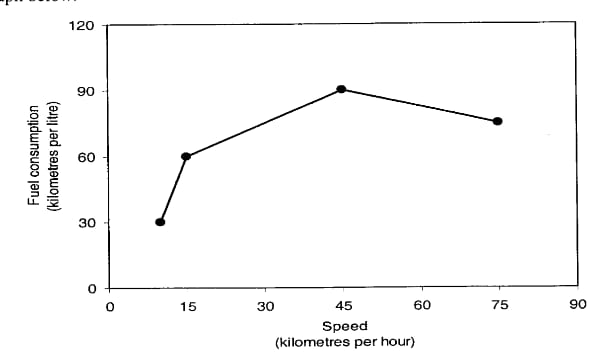
\includegraphics[width=7cm]{10}
	\caption*{}
	\label{fig:Q10}
	\end{figure}
The distances covered during four laps of the journey are listed in the table below
%TODO
%	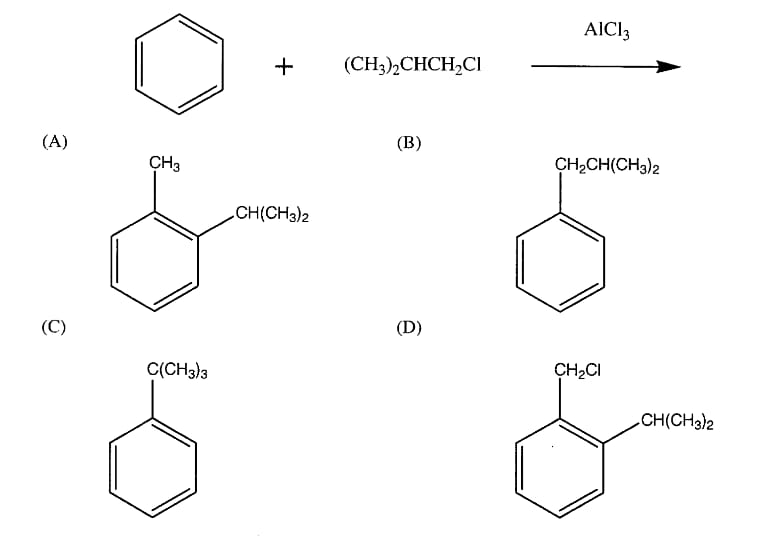
\includegraphics[width=\textwidth]{2}
From the given data, we can conclude that the fuel consumed per kilometre was least during the lap} 
\begin{table}[H]
\centering
	\begin{tabular}{|c|c|c|c|}
\hline
\text{Lap} & \text{Distance(kilometres)}  &\text{Average speed(kilometre per hour)} \\
\hline
P & 15 & 15\\
\hline
Q & 75 & 75 \\
\hline
R & 40 & 40 \\
\hline
S & 10 & 10\\
\hline
\end{tabular}

	\caption*{}
	\label{10}
\end{table}

	
		(A) P \hspace{10mm} (B) Q\hspace{10mm}(C) R\hspace{10mm}(D) S
\end{enumerate}\hfill{\textbf{GATE XL 2011}}
	

	\textbf{END OF THE SECTION - GA}
\newpage
	\textbf{H: CHEMISTRY (Compulsory)\newline Q. 1- Q. 5 carry one mark each.}
\begin{enumerate}
	\item{ Electrophile among the following is
		\begin{enumerate}
			\item{ $NH_3$}
			\item{ $SO_2$}
			\item{ $NO_2$}
			\item{$CH \equiv C^-$}

		\end{enumerate}\hfill{\textbf{GATE XL 2011}}
	\item{ The major product for the following reaction is}
	
	\begin{figure}[h!]
	\centering
	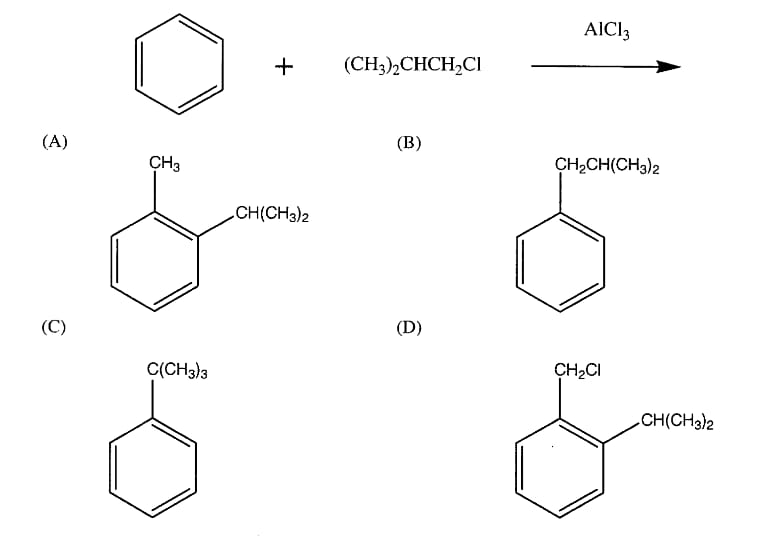
\includegraphics[width=\textwidth]{2}
	\caption*{}
	\label{fig:Q2}
	\end{figure}
	\item{ Trouton's rule is obeyed by}
		\begin{enumerate}
			\item{ hydrogen}
			\item{methanol}
			\item{benzene}
			\item{ acetic acid}

		\end{enumerate}\hfill{\textbf{GATE XL 2011}}
	\item{ Which one of the following compounds is known as silanes?}
		\begin{enumerate}
			\item{ Silicon hydrides}
			\item{ Silicon halides}
			\item{ Silicon hydroxides}
			\item{ Silicon oxides}

		\end{enumerate}\hfill{\textbf{GATE XL 2011}}

	\item{ The shape of PC1, is}
		\begin{enumerate}
			\item{ tetrahedral }
			\item{square planar }
			\item{trigonal bipyramidal}
			\item{square pyramidal}

		\end{enumerate}\hfill{\textbf{GATE XL 2011}}

%2011
	\textbf{Q. 6 - Q. 15 carry two marks each.}

	\item{ The correct order of acidity is}
		\begin{enumerate}
			\item{ $C_6H_5COOH < CH_3COOH < C_6H_5OH C_2H_5OH$}
		\item{$CH_3COOH < C_6H_5COOH < C_2H_5OH < C_6H_5OH$}
			\item{$C_2H_5OH < C_6H_5OH < C_6H_5COOH < CH_3COOH$}
			\item{$C_2H_5OH < C_6H_5OH< CH_3COOH < C_6H_5COOH$}

		\end{enumerate}\hfill{\textbf{GATE XL 2011}}

	\item{ Consider the following equilibrium \[ SO_2 (g) + \frac{1}{2} O_2 (g)\leftrightarrow SO_3 (g), \Delta H =-23.5 kCal mol_{-1} \]
		The formation of SO3 is favoured by}
		
		\begin{enumerate}
	\item{ compression and decreasing the temperature}

	\item{ compression and increasing the temperature}

	\item{ expansion and increasing the temperature }
	\item{ expansion and decreasing the temperature}
		\end{enumerate}\hfill{\textbf{GATE XL 2011}}

	\item {A molecular electronic excited state has a life time of 10$^{-9}$ s, the uncertainty in measuring the frequency (Hz) of the electronic transition is approximately}


		(A)$\frac{h}{4\pi} \times 10^{9}$ \hspace{10mm} (B) $\frac{h}{4\pi} \times 10^{-9}$\hspace{10mm}(C) $\frac{1}{4\pi} \times 10^{9}$\hspace{10mm}(D) $\frac{1}{4\pi} \times 10^{-9}$
	\item {According to the molecular orbital theory, bond order for H$_2^+$ species is}
	\begin{enumerate}
\item{ 0.5}
\item{ 1.0}

\item{ 1.5}

\item{ 2.0}
	\end{enumerate}\hfill{\textbf{GATE XL 2011}}


\item {According to crystal field theory, the electronic configuration of /Ti(H2O)/$_+$ in the ground state is}


(A) $e^1t^0_2$ \hspace{10mm} (B) $t^0_{2g}e_g^1$\hspace{10mm}(C) $e^0t^1_2$\hspace{10mm}(D) $t^1_{2g}e^0_g $

\item {The ions with lowest and highest radii among O$_2$, F, Na and Mg$^{2+}$ are respectively,}


		\begin{enumerate}
			\item{ $Mg^{2+} and O_2^-$}
			\item{ $O_2^- and Mg^{2+}$}
			\item{ $O_2^- and F$}
			\item{ $Na^+ and Mg^{2+}$}

		\end{enumerate}\hfill{\textbf{GATE XL 2011}}


\textbf{Common Data Questions}
\newline
\section{Common Data for Questions 12 and 13}

\subsection{The solubility products of FeS, ZnS, CuS and HgS are 1.0 x 10-19, 4.5 x 10-24, 4.0 x10-38 and 3.0 x 10-53 respectively.}`

\item {H$_2$S is passed through an aqueous solution containing all the four metal ions. The metal ion that precipitates first is}
	$(A) Fe^{2+} \quad (B) Zn^{2+} \quad(C) Cu^{2+} \quad(D) Hg^{2+}$}
\item {The concentration of S$_2-$, at which FeS begins to precipitate from the mixture having 0.1 M Fe$^{2+}$ is}
	\begin{enumerate}
\item{ 1.0 x 10$^{-7}$ M}

\item{ 1.0 x 10$^{-18}$ M}

\item{ 1.0 x 10$^{-19}$ M}

\item{ 1.0 x 10$^{-20}$ M}
	\end{enumerate}\hfill{\textbf{GATE XL 2011}}


\textbf{Linked Answer Questions}

\paragraph{Statement for Linked Answer Questions 14 and 15:}

Consider the reaction

	\begin{figure}[h!]
	\centering
		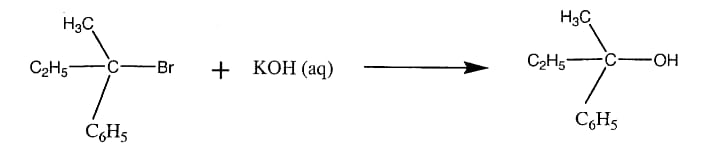
\includegraphics[width=10cm]{14}
	\caption*{}
	\label{fig:Q14}
	\end{figure}
\item {The above reaction is an example of}
		\begin{enumerate}
			\item{ addition reaction}
			\item{ bimolecular elimination reaction (E$_2$)}
			\item{ unimolecular substitution reaction (SN$_1$)}
			\item{ bimolecular substitution reaction (SN$_2$)}

		\end{enumerate}\hfill{\textbf{GATE XL 2011}}
	\item {If the concentration of KOH in the reaction mixture is doubled, the rate of the reaction will be}
		\begin{enumerate}
			\item{ decreased to one-half}
			\item{ the same }
			\item{ increased by two-times}
			\item{ increased by four-times}

		\end{enumerate}
		\hfill{\textbf{GATE XL 2011}}
\begin{center}
\textbf{END OF SECTION - H}
\end{center}
\end{enumerate}
\newpage

\begin{center}
\textbf{ I : BIOCHEMISTRY}

\textbf{Q. 1 - Q.10 carry one mark each.}

\end{center}
\begin{enumerate}
	\item {Which one of the following \textbf{DOES NOT} inhibit protein biosynthesis?} 
		\begin{multicols}{4}
		\begin{enumerate}
			\item Puromycin	
			\item Chloramphenicol	
			\item Cycloheximide	
			\item Ologomycin
		\end{enumerate}
		\end{multicols}
		\hfill{\textbf{GATE XL 2011}}
	\item {The activation of the complement components occurs via three distinct pathways. Which of the following component(s) is specific to the 'Alternate Pathway'?}
	\begin{enumerate}
			\item Factor B and ID
			\item Mannose binding protein
			\item C1qr2s2
			\item C2
		\end{enumerate}
		\hfill{\textbf{GATE XL 2011}}

	\item {Which one of the following enzymes fixes CO, into organic form?}
		\begin{enumerate}
			\item Ribulose 5-phosphate kinase
			\item Ribulose 1,5-bisphosphate carboxylase
			\item Pyruvate dehydrogenase
			\item Carbonic anhydrase
		\end{enumerate}
		\hfill{\textbf{GATE XL 2011}}

	\item {Cytochrome C is normally found in the inner mitochondrial membrane. It is released into the cytoplasm during}
	\begin{enumerate}
			\item Apoptosis
			\item Necrosis
			\item Cell differentiation
			\item Cell proliferation
		\end{enumerate}
		\hfill{\textbf{GATE XL 2011}}

	\item{ Horseradish peroxidase and alkaline phosphatase are the two enzymes commonly utilized as reagents in ELISA, because these enzymes}
		\begin{enumerate}
			\item are colored proteins
			\item are very small
			\item bind to ELISA plates
			\item have high turnover number
		\end{enumerate}
		\hfill{\textbf{GATE XL 2011}}

	\item {The polarity of water molecule is due to}
		\begin{enumerate}
			\item its tetrahedral structure
			\item honding electrons heing attracted more to oxygen 
			\item bonding electrons being attracted more to hydrogen
			\item its weak electrolytic property
		\end{enumerate}
		\hfill{\textbf{GATE XL 2011}}

	\item {Cyanide poisoning is due to its direct inhibition of}
		\begin{enumerate}
			\item Electron transport chain.
			\item Fatty acid biosynthesis
			\item Fatty acid oxidation
			\item Nucleic acid biosynthesis.
		\end{enumerate}
		\hfill{\textbf{GATE XL 2011}}

	\item{ In humans, the largest energy reserve is}
		\begin{enumerate}
			\item liver glycogen
			\item muscle glycogen
			\item blood glucose
			\item adipose tissue triacylglycerol
		\end{enumerate}
		\hfill{\textbf{GATE XL 2011}}

\item {A mixture of four proteins of pls 11, 7, 5 and 3 are loaded on DEAE anion-exchange column equilibrated with low ionic strength buffer of pH 8. Which of the four proteins would be expected to be retained on the column?}
		\begin{enumerate}
			\item Protein with pl 11 but not the others.
			\item Proteins with pls 11 and 7 but not 5 and 3
			\item Proteins with pls 7, 5 and 3
			\item Protein with pl 7 but not the others
		\end{enumerate}
		\hfill{\textbf{GATE XL 2011}}

\item {Valinomycin, a cyclic peptide antibictic, facilitates the transport of which one of the following ions?}
		\begin{enumerate}
			\item K$^+$
			\item Ca$^{2+}$
			\item Na$^+$
			\item H$^+$
		\end{enumerate}
		\hfill{\textbf{GATE XL 2011}}
\begin{center}
\textbf{Q. 11-Q. 20 carry two marks each.}
\end{center}
\item {Match P, Q, R and S with the appropriate numbers 1 to 6 on the right}

	\begin{minipage}{0.5\textwidth}
	\begin{flushleft}

		P) Basophils

Q) T cells.

R) B cells

S) Neutrophils

		\end{flushleft}
		\end{minipage}
	\begin{minipage}{0.5\textwidth}
		\begin{flushleft}
1) Perforin

2) Phagocytosis

3) Albumin

4) Macroglobulin

5) Fc receptors for IgE

6) Plasma cells
		\end{flushleft}
		\end{minipage}
		\begin{enumerate}
			\item P-5, Q-1, R-6, S-2
			\item P-1, Q-2, R-3, S-4
			\item P-3, Q-4, R-5. S-1
			\item P-2, Q-6, R-1, S-3
		\end{enumerate}
		\hfill{\textbf{GATE XL 2011}}

\item {Two purified DNA samples A and B contain equal number of basepairs. Each of these DNA samples has one site each for EcoRI and BamHI restriction enzymes. Complete digestion with both the enzymes yielded 3 DNA bands and 2 DNA bands respectively for A and B upon electrophoresis of the digestion products. Which one of the following explains the observation?}
	\begin{enumerate}
		\item{ A is circular DNA and B is linear}

		\item{ B is circular DNA and A is lincar}

		\item{ A is circular DNA and B could be linear or circular}

		\item{ B is circular DNA and A could be linear or circular}
	\end{enumerate}
	\hfill{\textbf{GATE XL 2011}}
\item {In the following enzyme catalyzed reaction which follows Michaelis-Menten kinetics	
	\textbf{ \[E + S \leftrightarrow ES \rightarrow E + P\]}
	
	$K_m$ is equal to}
		\begin{enumerate}
			\item $k_{-1}/(k_1k_2)$
			\item $(k_1. k_2)/k_{-1}$
			\item $ k_1/(k_2+k_{-1})$
			\item $(k_2+k_{-1})/k_1$
		\end{enumerate}
		\hfill{\textbf{GATE XL 2011}}

\item {Match the items in Group I with those in Group II}
	\newline
\begin{minipage}{0.5\textwidth}
\begin{flushleft}
	Group - I
P) Progesterone

Q) Dopamine

R) Vasopressin

5) Prostaglandin

		\end{flushleft}
		\end{minipage}
	\begin{minipage}{0.5\textwidth}
		\begin{flushleft}
Group II

1) Peptide

3) Carbohydrate

2) Fatty acid

4) Catecholamine

5) Eicosanoid

6) Steroid
		\end{flushleft}
		\end{minipage}


		\begin{enumerate}
			\item P-3, Q-4, R-1, S-2
			\item P-6, 0-4, R-1, 8-5
			\item P-3, Q-5, R-4, S-1
			\item P-6, Q-5, R-1, S-4
		\end{enumerate}
		\hfill{\textbf{GATE XL 2011}}

\item {Three samples of antibodies were electrophoresed under denaturing and reducing conditions on a 15\% acrylamide gel, followed by staining with Coomassie blue dye. Samples 1. 2 and 3 showed two, three and four stainable hands respectively. Which one of the following conclusions can be made from these observations?}
		\begin{enumerate}
			\item Sample 1 is IgG, 2 is IgA and 3 is IgM
			\item Sample 1 is IgA, 2 is IgM and 3 is IgG
			\item Sample 1 is IgA, 2 is IgM and 3 is IgG
			\item Sample 1 is IgA, 2 is IgG and 3 is IgM
		\end{enumerate}
		\hfill{\textbf{GATE XL 2011}}

\item {Four identical PCR reactions were carried out in tubes named I, II, III and IV. Besides the usual mix of dNTPs, each of the tubes respectively contained $\gamma^{32}P$dATP. $\beta-^{32}$P dATP, $\alpha-^{32}$P JATP and $\alpha - ^{32}$P INTP. Which one of the tubes will have radiolabeled PCR product?}


		\begin{enumerate}
			\item Tube I
			\item Tube II
			\item Tube III
			\item Tube IV
		\end{enumerate}
		\hfill{\textbf{GATE XL 2011}}

\item {Match the following:}


\begin{minipage}{0.5\textwidth}
\begin{flushleft}

Group I

P) Polynucleotide kinase

0) Fluoride

2) GTPase

R) Ras

S) lac operon

		\end{flushleft}
		\end{minipage}
	\begin{minipage}{0.5\textwidth}
		\begin{flushleft}
Group II

1) ATPase

3) Transketolase

4) Enolase

5) 5' end of DNA

6) 3' end of DNA

7) Only positive regulation

8) Positive and negative regulation
		\end{flushleft}
		\end{minipage}

		\begin{enumerate}
			\item P-5, Q-4, R-2, S-8
			\item P-6. Q-3, R-1. S-7
			\item P-4. Q-2, R-1, S-6
			\item P-1, Q-7, R-5. S-3
		\end{enumerate}
		\hfill{\textbf{GATE XL 2011}}

\item{Collagen, $\alpha$-keratin and tropomyosin have common structural features. They are

P) disulfide bridges to neighboring proteins.

Q) repeating sequences of amino acids

R) a high $\beta$-sheet content

S) superhelical coiling}
		\begin{enumerate}
			\item P.Q
			\item Q,R
			\item Q.S
			\item P.R
		\end{enumerate}
		\hfill{\textbf{GATE XL 2011}}

\item {Match the following}
	


\begin{minipage}{0.5\textwidth}
	\begin{flushleft}


Group I

P) Tyrosine hydroxylation.

(0) Tyrosine iodination.

R) Tyrosine phosphorylation

S) Tyrosine oxidation

		\end{flushleft}
		\end{minipage}
	\begin{minipage}{0.5\textwidth}
		\begin{flushleft}
Group II
1) Thyroxine


2) T cell Receptor


3) DOPA


4) Estradiol receptor

5) Epinephrine

6) Melanin

7) Endorphin

8) Serotonin
		\end{flushleft}
		\end{minipage}

		\begin{enumerate}
			\item P1, Q-6. R-5, S-4
			\item P-5, Q-7, R-4, 8-8
			\item P-2, Q-5, R-3, S-4
			\item P-3. Q-1, R-2, S-6
		\end{enumerate}
		\hfill{\textbf{GATE XL 2011}}

	\item {Scatchard analysis of ligand-receptor interaction yielded the graph shown below. The affinity of the ligand-receptor interaction can be obtained from}

	\begin{figure}[h!]
	\centering
	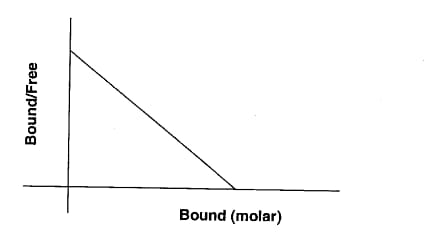
\includegraphics[width=\textwidth]{20}
	\caption*{}
	\label{fig:Q20}
	\end{figure}

		\begin{enumerate}
			\item Y intercept
			\item X intercept
			\item Slope of the line
			\item Product of X intercept and Y intercept
		\end{enumerate}
		\hfill{\textbf{GATE XL 2011}}

\end{enumerate}

\begin{center}
\textbf{END OF SECTION - I}
\end{center}
\newpage
\textbf{J: BOTANY}

\textbf{Q.1-Q. 10 carry one mark each.}
\begin{enumerate}
\item {The stalk with which the ovule remains attached to the placenta is called}


		\begin{enumerate}
			\item Micropyle
			\item Chalaza
			\item Funiculus
			\item Hilum
		\end{enumerate}
		\hfill{\textbf{GATE XL 2011}}

\item {The diploid chumosome number of an organism is 2n 14. What would be the expected chromosome numbers in a nullisomic?}
		\begin{enumerate}
			\item 12
			\item 13
			\item 15
			\item 16
		\end{enumerate}
		\hfill{\textbf{GATE XL 2011}}

\item {The mutagen ethidium bromide acts as a}

		\begin{enumerate}
			\item Deaminating agent
			\item Alkylating agent
			\item Intercalating agent
			\item Base analogue
		\end{enumerate}
		\hfill{\textbf{GATE XL 2011}}

\item{During photorespiration the reactive oxygen species. , is produced in}
		\begin{enumerate}
			\item Glyoxysome
			\item Lysosome
			\item Peroxisome
			\item Dictyosome
		\end{enumerate}
		\hfill{\textbf{GATE XL 2011}}

\item{ One of the defense mechanisms adopted by plants for detoxification of heavy metais is the synthesis of}
		\begin{enumerate}
			\item Phytochelatin
			\item Calmodulin
			\item Tubulin
			\item Systemin
		\end{enumerate}
		\hfill{\textbf{GATE XL 2011}}

	\item {In which one of the following phases of cell cycle the drug colchicine exerts its effect?}

		\begin{enumerate}
			\item GI
			\item G2
			\item S
			\item M
		\end{enumerate}
		\hfill{\textbf{GATE XL 2011}}

\item {The transition of water molecule from liquid to glassy state during cryopreservation is termed as Q.7}
		\begin{enumerate}
			\item Vitrification
			\item Hyperhydricity
			\item Cryoprotectant
			\item Habituation
		\end{enumerate}
		\hfill{\textbf{GATE XL 2011}}

	\item {The DNA content of a nucleus can be measured by}
		\begin{enumerate}
			\item ESR Spectroscopy
			\item FTIR Spectroscopy
			\item Flow Cytometry
			\item X-Ray Crystallography
		\end{enumerate}
		\hfill{\textbf{GATE XL 2011}}

\item {Retrograde signaling involves communication of}
	\begin{enumerate}
			\item nucleus to the chloroplast
			\item endoplasmic reticulum to the nucleus.
			\item nucleus to the mitochondria
			\item chloroplast to the nucleus
		\end{enumerate}
		\hfill{\textbf{GATE XL 2011}}

\item {A photoautotrophic micropropagation system can be established by increasing the}
		\begin{enumerate}
			\item sucrose concentration in the culture medium
			\item CO, concentration in the culture medium
			\item agar concentration in the culture medium
			\item NH$_3$ concentration in the culture medium.
		\end{enumerate}
		\hfill{\textbf{GATE XL 2011}}

\begin{center}
\textbf{Q. 11-Q. 20 carry two marks each.}
\end{center}
\item{Which of the following statements in photosynthesis are CORRECT?

P. The absorption maxima for photosystem I (PS I) and PS II are 680 nm and 700 nm, respectively Q. Photosynthetic reaction centre contains 300 chlorophyll molecules and the release of one

molecule of oxygen requires a minimum of 8 photons

R. The non-photochemical quenching of excitation energy is enhanced by the presence of

zeaxanthin

S. The photochemical splitting of water occurs in PS 1}
		\begin{enumerate}
			\item P. Q
			\item R, S
			\item P, S
			\item Q. R
		\end{enumerate}
		\hfill{\textbf{GATE XL 2011}}

\item {Which of the following statements are TRUE on DNA delivery methods during plant

transformation?

P. Single stranded nicks are made in T-DNA border repeat by the VirD1, VirD2 and VirD3 protein complex

Q. virA gene products form the export apparatus on the membrane for the transfer of T-DNA R. Gold/Tungsten particles are used as microprojectiles in biolistic method

S. Acceleration of DNA-coated microprojectiles is carried out with compressed CO}
		\begin{enumerate}
			\item P. S
			\item R. S
			\item P, R
			\item Q. S
		\end{enumerate}
		\hfill{\textbf{GATE XL 2011}}


\item {Match the following plant secondary compounds with their uses and source plants}



\begin{minipage}{0.3\textwidth}
	\begin{flushleft}

Compounds

P. Guggulusterol

Q. Shikonin

R. Ajmalicine

S. Glycyrrhizin


		\end{flushleft}
		\end{minipage}
		\begin{minipage}{0.3\textwidth}
		\begin{flushleft}

Uses

1. Anti-hypertensive
2. Anti-rheumatic

3. Dyc

4. Sweetner

5. Anti-tumor

6. Anti-plaque
		\end{flushleft}
		\end{minipage}
		\begin{minipage}{0.5\textwidth}
		\begin{flushleft}
Plant species


1. Lithospermum erythrorhizon

ii. Catharanthus roseus
iii. Glycyrrhiza glabra

iv. Commiphora wightii

v. Swertia chirata

vi. Coptis japonica

		\end{flushleft}
		\end{minipage}
	
		\begin{enumerate}
			\item P-4,Q-3,R-5,S-6
			\item P-4,Q-3,R-2,S-1
			\item P-2,Q-4,R-5,S-3
			\item P-4,Q-2,R-6,S-1
		\end{enumerate}
		\hfill{\textbf{GATE XL 2011}}

\item{Match the gene of interest for various aspects of crop improvement}
	

	\begin{minipage}{0.5\textwidth}
	\begin{flushleft}

Gene insert

P. bar

Q. vip3A

R. B-ley

S. gah-11

		\end{flushleft}
		\end{minipage}
	\begin{minipage}{0.5\textwidth}
		\begin{flushleft}


Aspects of crop improvement

1. Tolerance to heavy metals

2. Nutritional improvement with increased vitamin A

3. Insect resistance

4. Herbicide resistance

5. Delayed ripening

6. Resistance to fungal infection

		\end{flushleft}
		\end{minipage}

		\begin{enumerate}
			\item P-4,Q-3,R-5,S-6
			\item P-4,Q-3,R-2,S-1
			\item P-2,Q-4,R-5,S-3
			\item P-4, Q-2,R-6,S-1
		\end{enumerate}
		\hfill{\textbf{GATE XL 2011}}

\item {Match the plants with their seed storage proteins}


\begin{minipage}{0.5\textwidth}
	\begin{flushleft}


Plant

P. Rape seed

Q. Pea

R. Sorghum

S. Wheat

		\end{flushleft}
		\end{minipage}
	\begin{minipage}{0.5\textwidth}
		\begin{flushleft}

Protein

1. Kafirin

2. Viciilin

3. Gliadin

4. Napin

5. Zein

6. Patatin

		\end{flushleft}
		\end{minipage}


		\begin{enumerate}
			\item P-4,Q-3,R-5,S-2
			\item P-2,Q-3,R-6,S-1
			\item P-4,Q-2,R-1,S-3
			\item P-3,Q-2,R-2,S-5
		\end{enumerate}
		\hfill{\textbf{GATE XL 2011}}

\item {Match the name of the disease with the causal organism}

\begin{minipage}{0.5\textwidth}
	\begin{flushleft}
Causal organism

P. False smut of rice

Q. Ring rot of potato

R. Red rot of sugarcane

S. Downy mildew of grape



		\end{flushleft}
		\end{minipage}
	\begin{minipage}{0.5\textwidth}
		\begin{flushleft}

1. Plasmoparu viticola


2 Colletotrichum falcatum


3. Corynebacterium sepidonicum


4. Ustilaginoidea virens

5. Erwinia amylovora

6. Synchytrium endobioticum
		\end{flushleft}
		\end{minipage}

		\begin{enumerate}
			\item P-1, Q-5,R-2,S-4
			\item P-4,Q-3,R-2,S-1
			\item P-6,Q-2,R-4,S-1
			\item P-5,Q-3,R-2,S-4
		\end{enumerate}
		\hfill{\textbf{GATE XL 2011}}


\item {Identify the CORRECT statements for phylogenetic systems of classification.\newline P. The most popular phylogenetic systems of classification is that of George Bentham and Joseph Dalton Hooker and was published in 'Genera Plantarum

Q. A true phylogenetic system of classification was proposed by Adlof Engler and was published in 'Die Naturlichen Pflanzenfamilien'

R. The phylogenetic system of classification proposed by John Hutchinson was appeared in "The Families of Flowering Plants'

S. The origin of dicot from primitive monocot was proposed by Arthur Cronquist in his book 'Systema Naturae}

		\begin{enumerate}
			\item O. R
			\item P, Q
			\item R.S
			\item P. S
		\end{enumerate}
		\hfill{\textbf{GATE XL 2011}}

\item{ Which of the following statements are TRUE for the plastid genomes?

P. Plastid genome is circular in nature with genome size of 120-160 kb

Q. The plastid ribosomes are with sedimentation coefficient of 805

R. The gene for the small subunit of ribulose bisphospate carboxylase (RubisCO) is located in the plastid

S. rRNAs in the plastid genome are arranged in one transcription unit}
\begin{multicols}{4}
		\begin{enumerate}
			\item P,Q
			\item Q,S
			\item R,S
			\item P,S
		\end{enumerate}
\end{multicols}
		\hfill{\textbf{GATE XL 2011}}

\item {Identify the CORRECT statements.


P. Specialized parenchymatous celis with tannins and crystals of calcium oxalate are termed as sclereids

Q. The sieve elements of angiosperms are surrounded by companion cells and are essential component of phloem loading

R. The exudation of water by guttation occurs through trichomes

S. The bulliform cells control the unrolling and hygroscopic movement of grass leaves}

		\begin{enumerate}
			\item P,Q
			\item P,R
			\item Q,S
			\item P,S
		\end{enumerate}
		\hfill{\textbf{GATE XL 2011}}

\item {Which of the following statements are INCORRECT on ecological point of view?

P. Primary succession involving xerosere is initiated in a wet habitat

Q. Halones commonly found in electronic equipment are one of the active force destroying the protective ozone layer in the stratosphere

R. Sympatric speciation occurs when the new species evolves in geographic isolation from the parent species

S. a-Diversity is the diversity of specics within a habitat or community
}
		\begin{enumerate}
			\item P,Q
			\item P,R
			\item Q,R
			\item Q,S
		\end{enumerate}
\hfill{\textbf{GATE XL 2011}}



\textbf{END OF SECTION - J}
\end{enumerate}
\newpage
\textbf{K: MICROBIOLOGY}

\textbf{Q.1-Q. 10 carry one mark each.}
\begin{enumerate}
\item {Quinolones inhibit bacterial growth by targeting}
		\begin{enumerate}
			\item DNA replication
			\item mRNA translation
			\item RNA polymerase
			\item active transport of nutrients into the cell
		\end{enumerate}
		\hfill{\textbf{GATE XL 2011}}
\item {To select for spontaneously arising histidine auxotrophs in a population, you would use a medium containing}
		\begin{enumerate}
			\item Histidine and penicillin
			\item Penicillin but no histidine
			\item Histidine and lysozyme
			\item Lysozyme but no histidine
		\end{enumerate}
		\hfill{\textbf{GATE XL 2011}}
\item {Which one of the following statements is NOT associated with contributions of Louis Pasteur?}
		\begin{enumerate}
			\item Anthrax is caused by anthrax hacillus
			\item Bacteria causing food spoilage come from air
			\item The disease causing organism must be isolated in pure culture
			\item Bacteria cause the wine disease
		\end{enumerate}
		\hfill{\textbf{GATE XL 2011}}
\item {The active transport of solute in the cell is characterized by}
		\begin{enumerate}
			\item its uptake along the concentration gradient utilizing energy
			\item requirement of a carrier to support transport along the concentration gradient
			\item chemical modification of the solute during its uptake
			\item its uptake against the concentration gradient
		\end{enumerate}
		\hfill{\textbf{GATE XL 2011}}
\item {Catabolite repression allows cells to save energy by}
		\begin{enumerate}
			\item inactivating catabolic enzymes
			\item inhibiting synthesis of total RNA
			\item regulating expression of genes required for utilization of less-efficient metabolites.
			\item inhibiting translation of mRNAs encoding catabolic enzymes
		\end{enumerate}
		\hfill{\textbf{GATE XL 2011}}
	\item {A newly emerged variant of Influenza virus can be selectively propagated from the mixed population by addition of}

		\begin{enumerate}
			\item Gangcyclovir
			\item Tamiflu
			\item Interferon gamma
			\item Neutralizing antibody
		\end{enumerate}
		\hfill{\textbf{GATE XL 2011}}
\item {The synthesis of an immunoglobulin in either a secretory or membrane bound form is governed by}
		\begin{enumerate}
			\item allelic exclusion
			\item class switching
			\item differential RNA processing
			\item affinity maturation.
		\end{enumerate}
		\hfill{\textbf{GATE XL 2011}}
\item {The cis-trans test can determine whether a gene codes for}
		\begin{enumerate}
			\item an activator or a repressor
			\item an RNA or a protein
			\item a protein with the same or different amino acids
			\item a diffusible or non-diffusible product
		\end{enumerate}
		\hfill{\textbf{GATE XL 2011}}
\item {Which of the following are expected to be the abundant inhabitants of a nitrate and sulfate rich soil naturally depleted for oxygen?}
		\begin{enumerate}
			\item Pseudomonas and Azotobacter
			\item Pseudomonas and Desulfovibrio
			\item Azotobacter and Thiobacillus
			\item Nitrosomonas and Nitrobacter
		\end{enumerate}
		\hfill{\textbf{GATE XL 2011}}
\item{ Which one of the following immersion oils would you use to get the best resolution in a light microscope (with 100X objective)?}
		\begin{enumerate}
			\item an oil with refractive index of 1.6
			\item an oil with refractive index of 1.5
			\item an oil with refractive index of 1.4
			\item an oil with refractive index of 1.3
		\end{enumerate}
		\hfill{\textbf{GATE XL 2011}}
\begin{center}
\textbf{Q. 11-Q. 20 carry two marks each.}
\end{center}
\item {Four Hfr strains of E. coli were generated from the same F strain. The Hfr strains donated markers in the following order

Strain1: DQWMT; Strain 2: AXPTM; Strain 3: BNCAX; Strain 4: BDOWM

The order of the markers in the original F" strain is}
		\begin{enumerate}
			\item DQWMTPXACNB
			\item AXPTMDQWBNC
			\item BNCAXPTMDOW
			\item BDQWMNCAXPT
		\end{enumerate}
		\hfill{\textbf{GATE XL 2011}}
\item {Which one of the following forms of the same DNA molecule would bind maximum ethidium bromide?}
		\begin{enumerate}
			\item Negatively supercoiled.
			\item Covalently closed relaxed circle
			\item Linear
			\item Positively supercoiled
		\end{enumerate}
		\hfill{\textbf{GATE XL 2011}}
\item {An actively growing culture of E. coli divides in about 20 min. Under laboratory conditions, time taken to replicate the entire genome of this bacterium would be about}
		\begin{enumerate}
			\item 20 min
			\item 40 min
			\item 10 min
			\item 18 min
		\end{enumerate}
		\hfill{\textbf{GATE XL 2011}}
\item {Which of the statements about Corynebacterium diphtheriae biology is NOT CORRECT?}
		\begin{enumerate}
			\item All strains of C. diphtheriae are producers of diphtheria toxin
			\item Diphtheria toxin production can be minimized by high concentration of iron in the medium
			\item Diphtheria toxin inhibits protein synthesis
			\item Diphtheria toxin is an A-B toxin secreted as a polypeptide of 62 kDa
		\end{enumerate}
		\hfill{\textbf{GATE XL 2011}}
\item {Match the names of investigators in Group 1 with their contributions in Group 2}


	\begin{minipage}{0.5\textwidth}
	\begin{flushleft}


Group 1

P. Joseph Lister

Q. John Needham

R. Elie Metchnikoff

S. Lazaro Spallanzani
		\end{flushleft}
		\end{minipage}
	\begin{minipage}{0.5\textwidth}
		\begin{flushleft}

Group 2

1. Role of phagocytosis in infection


2. Disproved spontaneous generation


3. Proved Spontaneous generation


4. Use of agar as solidifying agent

5. Use of carbolic acid as disinfectant
		\end{flushleft}
		\end{minipage}

\begin{multicols}{4}
		\begin{enumerate}
			\item P-5,Q-3.R-4.S-1
			\item P-5,Q-3,R-1,S-2
			\item P-4.Q-3R-1,S-5
			\item P-3,Q-2,R-1.5-4
		\end{enumerate}
\end{multicols}
		\hfill{\textbf{GATE XL 2011}}

	\item {During replication of the E. coli chromosome, Okazaki fragments are produced from}

		\begin{enumerate}
			\item only one of the strands of the circular genome
			\item both the strands of the circular genome
			\item one of the strands in one generation and the other strand in the next generation
			\item both the strands of the circular genome provided that the heavy nitrogen ("N) is present in the medium
		\end{enumerate}
		\hfill{\textbf{GATE XL 2011}}

\item {A new isolate of a facultative anaerobe utilizes either oxygen or pyruvate as terminal electron acceptor. This bacterium was grown either anaerobically with glucose as sole carbon source, or aerobically with lactose as the sole carbon source. Net increase in ATP production (par mole of the carbon source) during the aerobic growth would be}
		\begin{enumerate}
			\item 2-fold
			\item 4-fold
			\item 19-fold
			\item 38-fold
		\end{enumerate}
		\hfill{\textbf{GATE XL 2011}}
\item {Based on their properties, match the "Genera" in Group 1 with those in Group 2}


	\begin{minipage}{0.5\textwidth}
	\begin{flushleft}


Group 1

P. Bacillus

Q. Neisseria

R. Rhizobium

S. Caulabacter
		\end{flushleft}
		\end{minipage}
	\begin{minipage}{0.5\textwidth}
		\begin{flushleft}

Group 2

1. Sarcina

2. Azotobacter

3. Hyphomicrobium

4. Clostridium
		\end{flushleft}
		\end{minipage}


		\begin{enumerate}
			\item P-4, Q-1.R-2,5-3
			\item P-4, Q-1,R-3,5-2
			\item P-2, Q-4.R-1.S-3
			\item P-1. Q-4.R-2,S-3
		\end{enumerate}
		\hfill{\textbf{GATE XL 2011}}

\item {An actively growing culture (20 ml) of E. coli (1 x 10 per ml) was mixed with a total of 100 T4 phage particles, grown further for 40 min and mixed with a few drops of chloroform. Under the conditions used, the generation time of E. coli is 30 min, the infection cycle of phage T4 is 20 min, and the burst size is 100). Assuming that each infection was a successful one, how many plaque forming units would you expect at the end of the experiment?}
		\begin{enumerate}
			\item 10$^4$
			\item 10$^3$
			\item 10$^5$
			\item 10$^6$
		\end{enumerate}
		\hfill{\textbf{GATE XL 2011}}
\item {Match the pair of organisms in Group 1 with their characteristic interactions in Group 2}
\newline
\begin{minipage}{0.5\textwidth}
	\begin{flushleft}

Group 1

P. Photoblepharon palpebratus and Vibrio fischeri

Q. Pseudomonas and Bdellavibrio

R. Aspergillus and Pseudomonas
S. Thiobacillus ferrooxidans and Beijerinckia lacticogenes

		\end{flushleft}
		\end{minipage}
	\begin{minipage}{0.5\textwidth}
		\begin{flushleft}

Group 2
1. Mutualism

2. Symbiosis.


3. Antagonism


4. Parasitism
		\end{flushleft}
		\end{minipage}


		\begin{enumerate}
			\item P-2,Q-4.R-3.S-1
			\item P-2,Q-3.R-4,S-1
			\item P-4.Q-2,R-3,5-1
			\item P-2,0-4,R I.S 3
		\end{enumerate}
		\hfill{\textbf{GATE XL 2011}}

\textbf{END OF SECTION-K}

\end{enumerate}
\newpage
		\textbf{L: Zoology}

\textbf{Q.1-Q. 10 carry one mark each.}

\begin{enumerate}
	\item{ Which one of the following is an example of eumetazoans?}
		\begin{enumerate}
			\item Dictyostelium
			\item Hydra
			\item Sponges
			\item Volvox
		\end{enumerate}
		\hfill{\textbf{GATE XL 2011}}
		
	\item {Which one of the following is characteristic of deuterostomes?}

		\begin{enumerate}
			\item Radially symmetric body
			\item Bilaterally symmetric body
			\item Presence of well-defined digestive system
			\item Formation of anus from blastopore
		\end{enumerate}
		\hfill{\textbf{GATE XL 2011}}

	\item{ Extraembryonic tissues are derived from which one of the following?}
		\begin{enumerate}
			\item Ectoderm
			\item Endederm
			\item Trophocctoderm
			\item Mesoderm
		\end{enumerate}
		\hfill{\textbf{GATE XL 2011}}
		
	\item{ Which one of the following type of immune cells is responsible for graft rejection?}

		\begin{enumerate}
			\item B cells
			\item T cells
			\item Macrophages
			\item Eosinophils
		\end{enumerate}
		\hfill{\textbf{GATE XL 2011}}
		
	\item{ Which of the following is a main symptom of infection by Wuchereria bancrofti?}
		\begin{enumerate}
			\item Swelling of limbs
			\item Skin rashes
			\item Blindness
			\item Brain cyst
		\end{enumerate}
		\hfill{\textbf{GATE XL 2011}}
		
	\item{ In insect's tracheal system, the transport of oxygen to the target tissue is done by}
		\begin{enumerate}
			\item fine branches of air tubes extending to almost every cell
			\item a liquid that fills the tracheal tube
			\item a specialized set of cells that produce myoglobin
			\item a specialized pigment
		\end{enumerate}
		\hfill{\textbf{GATE XL 2011}}
\item {Which one of the following examples represents an adaptation or a physiological activity that DOES NOT minimize the loss of body temperature of animals?}
		\begin{enumerate}
			\item Feathers or fur
			\item Fat layers in the adipose tissue
			\item Shivering
			\item Vasodilation
		\end{enumerate}
		\hfill{\textbf{GATE XL 2011}}

	\item{ Which one of the following hormones is INCORRECTLY paired with its function?}
		\begin{enumerate}
			\item Melatonin-biological rhythm
			\item Glucagon-increases blood glucose levels
			\item Prolactin-stimulates milk secretion.
			\item Calcitonin-increases blood calcium level
		\end{enumerate}
		\hfill{\textbf{GATE XL 2011}}

\item{ The term innate behavior refers to an animal behavior}
		\begin{enumerate}
			\item that is triggered by an environmental change
			\item that is taught by the parent
			\item that is developmentally fixed
			\item that an organism learns on its own by "a hit-and trial" approach
		\end{enumerate}
		\hfill{\textbf{GATE XL 2011}}
\item{ Which of the following is TRUE about Kreb's cycle?}
		\begin{enumerate}
			\item Kreb's cycle generates NADPH
			\item The enzymes of Kreb's cycle reside in the inter-membrane space of a mitochondria
			\item It produces ATP, the energy currency of a cell
			\item None of the above
		\end{enumerate}
		\hfill{\textbf{GATE XL 2011}}
\begin{center}
\textbf{Q. 11-Q. 20 carry two marks each.}
\end{center}
\item{ A genetic experiment was performed to map the gene(s) for eye colour in a newly-discovered moth species. Sex determination in this moth species: XY male and XX female. When blue-eyed males were mated to green-eyed females, all of both male and female progeny had green eyes. When these progeny were mated among themselves, about half of the males of the resulting second generation had blue eyes; however, all females were green-eyed. Which one of the following is consistent with the above data?}
		\begin{enumerate}
			\item Multiple genes control eye colour in this moth species
			\item Gene(s) for eye for eye colour is located on the X chromosome
			\item Gene(s) for eve colour is located on the Y chromosome
			\item Gene(s) for eye colour may not be sex-linked
		\end{enumerate}
		\hfill{\textbf{GATE XL 2011}}

\item {In a newly discovered organism, normal development was unaffected when a few blastomeres were removed from 100-cell stage embryo. However, removal of five cells at the 1000-cell stage abolished the formation of kidney. Which one of the following options most accurately describes the type(s) of specification operating in the development of this organism?}
\begin{enumerate}
	\item Conditional specification only
	\item Autonomous specification only
	\item Conditional and autonomous specifications
	\item Specification does not occur in this organism
\end{enumerate}
\hfill{\textbf{GATE XL 2011}}

\item{ In which one of the following organisms, it is easiest to distinguish mutations on adjacent base pairs of DNA through genetic recombination experiments?}

\begin{enumerate}
	\item Bacteriophages
	\item Yeast
	\item Escherichia coli
	\item Bacillus subtilis
\end{enumerate}
\hfill{\textbf{GATE XL 2011}}

\item{ RNA is considered as the first genetic material to have evolved on the earth. Which one of the following properties of RNA is critical for its functioning as the genetic material in the absence of DNA and protein?}

\begin{enumerate}
	\item The presence of uracil as a base in place of thymine
	\item The RNA is less stable than DNA; therefore RNA has higher probability to evolve as genetic material as compared to DNA
	\item The single stranded RNA has a genotype as well as phenotype
	\item RNA exists in 3 forms while DNA has only one form
\end{enumerate}
\hfill{\textbf{GATE XL 2011}}

\item{ The birth control pills contain hormonal formulations that may either arrest the ovulation or prevent the fertilization of egg. Some of the formulations do both. Which one of the following combinations represents formulation that is likely to affect the process of ovulation and fertilization?}

\begin{enumerate}
	\item Progesterone and estrogen
	\item Prostaglandin and estrogen
	\item Gonadotrophin and estradiol
	\item Prolactin and estradiol
\end{enumerate}
\hfill{\textbf{GATE XL 2011}}

\item {Behavioral studies on animals have shown that there is relationship between mechanism of reproduction and male parental care (protecting eggs or the young ones). In aquatic invertebrates, fishes and amphibians for example, the species that practice internal fertilization rarely show male parental care while a majority of species that practice external fertilization tend to exhibit male parental care. This is likely due to}

\begin{enumerate}
	\item the male sex in species that practice internal fertilization are unable to defend against the predators
	\item the male sex in species that practice internal fertilization live on female as parasite
	\item the fact that the females of species that practice external fertilization die soon after laying the eggs
	\item the certainty of paternity in species that practice external fertilization and this behavior is reinforced over generation by natural selection
\end{enumerate}
\hfill{\textbf{GATE XL 2011}}

\item{ The term biological magnification refers to the increased levels of a toxin seen in successive trophic levels in a food web. Which one of the following options correctly states the reason(s) for the increment of a toxin in the ecosystem?}
\begin{enumerate}
	\item The toxin is highly toxic to primary producers, relatively less toxic to primary consumers, and non-toxic to secondary consumers. Thus, a higher level of toxin is seen in species representing higher trophic levels.
	\item The toxin cannot be degraded by microorganism and consequently persist in the environment for years
	\item The toxin to begin with was not toxic or less toxic, but became more toxic by metabolism in the primary producers
	\item Both (B) and (C)
\end{enumerate}
\hfill{\textbf{GATE XL 2011}}

\item {From the point of view of the enzymatic reactions, which of the following DOES NOT belong here?}

\begin{enumerate}
	\item Telomerase
	\item Reverse transcriptase
	\item Taq polymerase
	\item Primase
\end{enumerate}
\hfill{\textbf{GATE XL 2011}}

\item{ Which of the following statements is/are TRUE about JUXTACRINE signaling?

I. The ligand and the receptor engage in reciprocal signaling

II. Both the ligand and the receptor are membrane associated proteins

III. The ligand gets proteolytically cleaved after binding to the receptor}

\begin{enumerate}
	\item I only
	\item II only
	\item III only
	\item I, II and II
\end{enumerate}
\hfill{\textbf{GATE XL 2011}}

\item{ Which of the following amino acid change (mutation) would MOST adversely affect the structure of an $\alpha$-helix?}
\begin{enumerate}
	\item A valine residue changed to an isoleucine residue 
	\item A methionine residue changed to a proline residue
	\item An aspartic acid residue changed to a glutamic acid residue
	\item A histidine residue changed to an arganine residue
\end{enumerate}
\hfill{\textbf{GATE XL 2011}}

\begin{center}
\textbf{END OF SECTION-L}
\end{center}
\end{enumerate}
\newpage
\textbf{M: FOOD TECHNOLOGY}

		\textbf{Q.1-Q. 10 carry one mark each.}

\begin{enumerate}
	\item{ The protein responsible for spongy structure in bread is}
\begin{enumerate}
	\item Albumin
	\item Zein
	\item Gluten
	\item Gliadin
\end{enumerate}
\hfill{\textbf{GATE XL 2011}}
	\item{ The factor most responsible for making a good ice cream is}
\begin{enumerate}
	\item Water content 
	\item Homogenization
	\item Emulsifying agent
	\item Mixing index
\end{enumerate}
\hfill{\textbf{GATE XL 2011}}
	\item{ Listed below are some of the functions of fats in the human nutrition. Identify the INCORRECT function}
\begin{enumerate}
	\item Concentrated source of energy
	\item Transport of oxygen to various organs
	\item Absorption of fat soluble vitamins
	\item Synthesis of cell membrane and hormones
\end{enumerate}
\hfill{\textbf{GATE XL 2011}}
	\item{ During ripening of cheese by Penicillium roqueforti the characteristic aroma is because of}
\begin{enumerate}
	\item
(A) Methyl ketones
	\item
(B) Aceto acetic acid
	\item
(C) Diacetyl
	\item
(D) Acetoin
\end{enumerate}
\hfill{\textbf{GATE XL 2011}}
	\item {Which of the following statements is NOT TRUE in case of oxidative rancidity of fatty foods?}
\begin{enumerate}
	\item Peroxides and hydroperoxides are formed during auto-oxidation
	\item Auto-oxidation is a complex chain reaction
	\item The final breakdown products of auto-oxidation are aldehydes, ketones and alcohols
	\item The reaction is brought about by an enzyme, called lipase
\end{enumerate}
\hfill{\textbf{GATE XL 2011}}
	\item{ Which of the following group of characteristics is CORRECT in respect of Shigella species found as food pathogen?}
\begin{enumerate}
	\item Gram positive, motile by gliding, spore forming cocci and transmitted by contaminated food
	\item Gram negative, motile by flagella, spore forming bacilli and transmitted by contaminated water
	\item Gram positive, non-motile, non-spore forming cocci and transmitted by contaminated air and water both
	\item Gram negative, non-motile, non-spore forming and transmitted by fecal-oral route
\end{enumerate}
\hfill{\textbf{GATE XL 2011}}
	\item {Relate the vitamins listed below (left hand side) with the associated diseases (right hand side)}
		\newline
\begin{minipage}{0.5\textwidth}
	\begin{flushleft}

P. Thiamin

Q. Nicotinic acid

R. Folic acid
S. Ascorbic acid
		\end{flushleft}
		\end{minipage}
	\begin{minipage}{0.5\textwidth}
		\begin{flushleft}
1. Pellagra

2. Beriberi

3. Scurvy

4. Anemia
		\end{flushleft}
		\end{minipage}

\begin{enumerate}
	\item P-1.Q-2.R-3, S-4
	\item P-4, Q-3, R-2,S-1
	\item P-2.Q-1,R-4.5-3
	\item P-3, Q-4, R-1, S-2
\end{enumerate}
\hfill{\textbf{GATE XL 2011}}

\item{ Which of the following conditions for the heat resistance of microorganisms is CORRECT?}

\begin{enumerate}
	\item $Psychrophiles < Mesophiles < Thermophiles$
	\item $Psychropniles > Mesophiles > Thermophiles$
	\item $Thermophiles > Psychrophiles > Mesophiles$
	\item $Mesophiles <Thermophiles < Psychrophiles$
\end{enumerate}
\hfill{\textbf{GATE XL 2011}}
\item{ The solubility of sodium bicarbonate in water is 9,6 g/100 g at 20 °C and 16.4 g/100 g at 60 "C. If a saturated solution of sodium bicarbonate at 60 °C is cooled to 20 °C, the percentage of the dissolved salt crystallized out will be}

\begin{enumerate}
	\item 20.5
	\item 25.4
	\item 41.5
	\item 45.2
\end{enumerate}
\hfill{\textbf{GATE XL 2011}}

\item {Which one of the following statements is NOT TRUE in terms of nutritive evaluation of proteins?}

\begin{enumerate}
	\item PER is defined as the live weight gain per unit weight of protein intake
	\item 'Metabolic nitrogen' is the amount of nitrogen present in the feces when a nitrogen free dies is fed to an animal
	\item Net protein utilization is a product of biological value and digestibility
	\item 'Chemical score' of a mixed protein diet can be calculated from the total amino acids present in the mixture
\end{enumerate}
\hfill{\textbf{GATE XL 2011}}
\begin{center}
\textbf{Q. 11-Q. 20 carry two marks each.}
\end{center}
\item {A sugar syrup (density 1040 kg/m$^3$ and viscosity = 1600 x 10$^{-6}$ Pas) is required to be pumped into a tank (1.5 m diameter and 3 m height) by a 3 cm inside diameter pipe. If the liquid is required. to flow under laminar conditions the minimum time to fill the tank with the syrup will be}
\begin{enumerate}
	\item 192.9 h
	\item 19.3 h
	\item 38.6 h
	\item 57.9 h
\end{enumerate}
\hfill{\textbf{GATE XL 2011}}
\item {Match the following sauerkraut defects for their causative agents}
\newline
	\begin{minipage}{0.5\textwidth}
	\begin{flushleft}


P. Soft kraut


Q. Slimy kraut

R. Rotted kraut

S. Pink kraut

		\end{flushleft}
		\end{minipage}
	\begin{minipage}{0.5\textwidth}
		\begin{flushleft}

1. Due to growth of bacteria, mold and/or yeast

2. Due to surface growth of Torula yeast


3. Bacterial growth does not initiate till last stage


4. Rapid growth of Lactobacillus cucumens and L. plantarum specially at elevated temperature

		\end{flushleft}
		\end{minipage}

\begin{enumerate}
	\item P-4.0-2.R-3,S1
	\item P-3, 0-4, R-1.S-2
	\item P-1, Q 3, R-2, S-4
	\item P-2.0-1.R-4.S-3
\end{enumerate}
\hfill{\textbf{GATE XL 2011}}

\item {Match the following carbohydrates with their use in the food processing}



	\begin{minipage}{0.5\textwidth}
	\begin{flushleft}

P. High amylose starch

Q. Pectin

R. Starch phosphates

S. Glucose


		\end{flushleft}
		\end{minipage}
	\begin{minipage}{0.5\textwidth}
		\begin{flushleft}

1. White sauces in cook freeze operations

2. Edible film for wrapping candies


3. As humectant in confectionary

4. Setting agent in jams and jellies
		\end{flushleft}
		\end{minipage}

\begin{enumerate}
	\item P-1,0-2, R-4, S-3
	\item P-2.Q-4, R-1, S-3
	\item P-3.Q-1,R-2. S-4
	\item P-4.Q-3, R-1, S-2
\end{enumerate}
\hfill{\textbf{GATE XL 2011}}

\item {Match the food items and their principal flavouring agents given in the two columns below.}
	\newline
\begin{minipage}{0.5\textwidth}
	\begin{flushleft}

P. Butter

Q. Orange


R. Cloves

S. Mint
		\end{flushleft}
		\end{minipage}
	\begin{minipage}{0.5\textwidth}
		\begin{flushleft}
1. Menthol


2. Limonene


3. Eugenol


4. Diacetal
		\end{flushleft}
		\end{minipage}
\begin{enumerate}
	\item P-3.0-2, R-4.5-1
	\item P-2, Q-3. R-1, S-4
	\item P-4, Q1, R-3, S-2
	\item P-4.Q-2, R-3.S-1
\end{enumerate}
\hfill{\textbf{GATE XL 2011}}


\item{ Match the food items on left hand side with their colloidal nature on right hand side}
	\newline
\begin{minipage}{0.5\textwidth}
	\begin{flushleft}

P. Curd

Q. Butter

R. Vegetable soup
S. Whipped egg white

		\end{flushleft}
		\end{minipage}
	\begin{minipage}{0.5\textwidth}
		\begin{flushleft}
1. Foam


2. Emulsion


3. Sol


4. Gel
		\end{flushleft}
		\end{minipage}

\begin{enumerate}
	\item P-2 Q-1, R-3.S-4
	\item P-4, Q3, R-2, S-1
	\item P-4, Q-2, R-3, S-1
	\item P-3, Q-4, R-1, S-2
\end{enumerate}
\hfill{\textbf{GATE XL 2011}}

\item{ In an actively growing (exponential phase) yeast culture, the cell concentration increased from 10 cells per ml to 10 \^ r cells per ml in 4 h. The doubling time of the yeast is}

\begin{enumerate}
	\item 120 minutes
	\item 30 minutes
	\item 18 minutes
	\item 60 minutes
\end{enumerate}
\hfill{\textbf{GATE XL 2011}}

\item{ The steps followed in Gram's staining of microorganisms are

P. Washing with neutral organic solvent

Q. Counter staining with a contrast dye

S. Fixing the colour with a suitable mordant

R. Staining with basic dye

Identify the CORRECT sequence.}
\begin{enumerate}
	\item QSRP
	\item PQRS
	\item QPSR
	\item RSPQ
\end{enumerate}
\hfill{\textbf{GATE XL 2011}}
\item{ A continuous dryer was used to dry 12 kg/min of a blanched vegetable containing 50\% moisture (wet weight basis) to give a product containing 10\% moisture. As the dryer could handle feed material with moisture content not more than 25\%, a part of dried material was recycled and mixed with the fresh feed. The evaporation rate in the dryer will be}
\begin{enumerate}
	\item 2.08kg / min
	\item 5.33kg / min
	\item 3.33 kg/min
	\item 2.93kg / min
\end{enumerate}
\hfill{\textbf{GATE XL 2011}}
\item {An enzyme has a K$_m$ of 4.7 $\times 10 ^{- 5}$ M and V$_m$ is 22 micro moles per litre per min. The enzyme reaction is carried out at a substrate concentration of $2 \times 10^ 4$ The initial reaction velocity for this enzyme catalyzed reaction will be}
\begin{enumerate}
	\item 6.5 micro moles per litre per min
	\item 17.8 micro moles per litre per min
	\item 13.0 micro moles per litre per min
	\item 8.9 micro moles per litre per min
\end{enumerate}
\hfill{\textbf{GATE XL 2011}}
\item {The F - value at 121.1 °C, equivalent to 99.9999 percent destruction of a strain of Clostridium bondinum, is 1.8 min. The D, value (decimal reduction time at reference temperature) of the organism will be}
\begin{enumerate}
	\item 10.8 min
	\item 0.3 min
	\item 6.0 min
	\item 0.2 min
\end{enumerate}
\hfill{\textbf{GATE XL 2011}}
\begin{center}
\textbf{END OF THE QUESTION PAPER}
\end{center}


\end{enumerate}
\end {document}
